\documentclass{beamer}
\usepackage{xeCJK}
\usetheme{Madrid}%简约
\usepackage{hyperref}

\begin{document}

\title{中国海洋大学}
\author{张中瑞}
\date{\today}

%图片
\begin{frame}
     \begin{figure}
     \centering 
     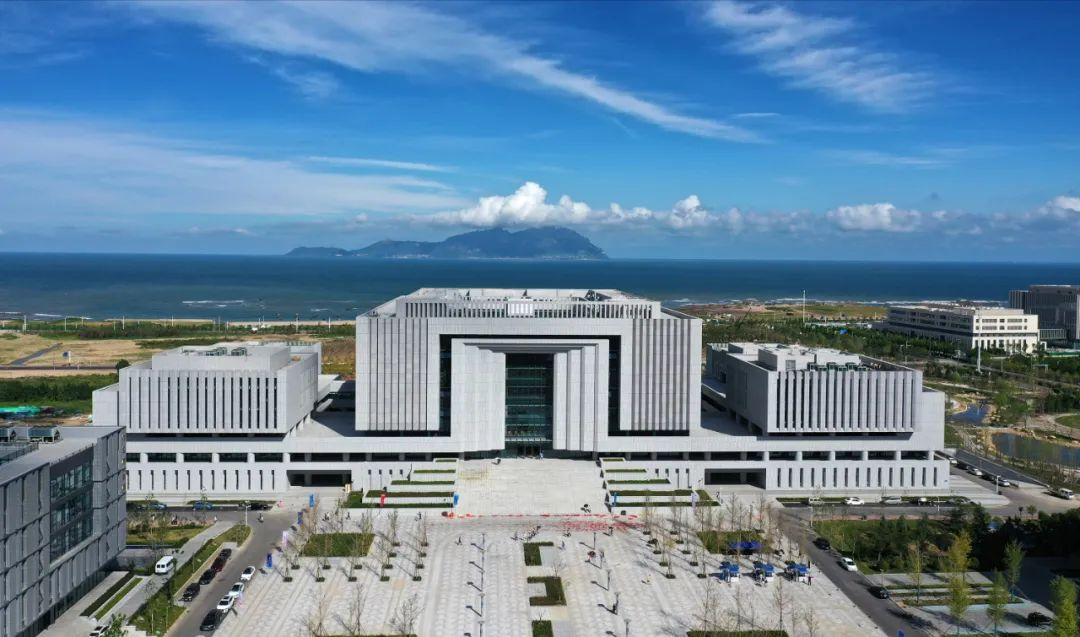
\includegraphics[width=0.8\textwidth]{R-C.jpg}
     \caption{中国海洋大学西海岸校区}
     \end{figure}
\end{frame}

%学校介绍
\begin{frame}{一、学校概况}
  \begin{itemize}
   \item 始建于1924年,前身为私立青岛大学
   \item 国家"双一流"A类建设高校,以海洋、水产为特色
   \item 拥有崂山、鱼山、浮山、西海岸四个校区
   \item 校训：\textbf{海纳百川、取则行远}%加粗
  \end{itemize}
\end{frame}

\begin{frame}{二、学科与科研}
   \begin{block}{1.王牌学科}
   2个"双一流"建设学科:\textbf{海洋科学}、\textbf{水产}(均为全国顶尖)
   \end{block}+
   \begin{block}{2.科研平台}
   拥有国家重点实验室、"科学"号海洋科考船等顶尖科研资源
   \end{block}
\end{frame}

\begin{frame}{三、学校定位}
   \centering
   \Large 中国海洋领域高层次人才培养基地 \\
   \Large 高水平海洋科学研究平台 \\
   \vspace{1cm}
   \small 官网：{https://www.ouc.edu.cn/}
\end{frame}

\end{document}
